\documentclass[tikz,border=2pt,11pt]{standalone}
\usetikzlibrary{arrows.meta}
\usetikzlibrary{calc}
\usepackage{amsmath}
\usepackage{amssymb}
\usepackage{tikz}
\newcommand{\R}{\mathbb R}
\newcommand{\N}{\mathbb N}
\newcommand{\eps}{\varepsilon}
\newcommand{\T}{T}
\newcommand{\dd}{\,\mathrm d}
\DeclareMathOperator{\conv}{conv}
\DeclareMathOperator{\supp}{supp}
\DeclareMathOperator{\dist}{dist}
\DeclareMathOperator{\diam}{diam}
\DeclareMathOperator{\Vol}{Vol}
\begin{document}
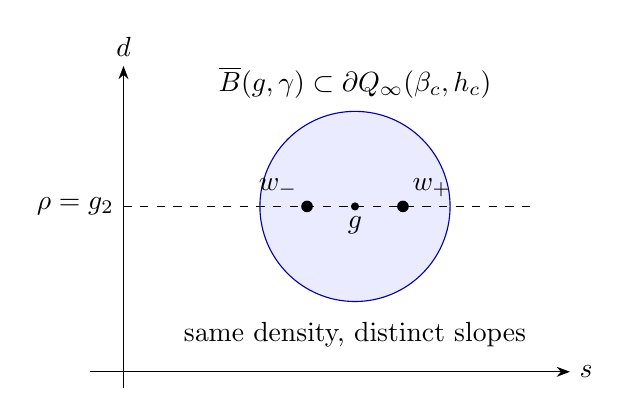
\begin{tikzpicture}[scale=1.05,>=Stealth]
 \draw[->] (-0.4,0) -- (5.4,0) node[right] {$s$};
 \draw[->] (0,-0.2) -- (0,3.7) node[above] {$d$};
 \fill[blue!8] (2.8,2) circle (1.15);
 \draw[blue!65!black] (2.8,2) circle (1.15);
 \draw[dashed] (0,2) node[left] {$\rho=g_2$} -- (5.0,2);
 \fill (2.8,2) circle (1.4pt) node[below] {$g$};
 \fill (2.22,2) circle (2pt) node[above left] {$w_-$};
 \fill (3.38,2) circle (2pt) node[above right] {$w_+$};
 \node[align=center] at (2.8,0.45) {same density, distinct slopes};
 \node at (2.8,3.5) {$\overline B(g,\gamma)\subset\partial Q_\infty(\beta_c,h_c)$};
\end{tikzpicture}
\end{document}
